In task 3 we want to take the vehicle dynamics linearized about the (optimal) trajectory $(x_{opt}, u_{opt})$ computed in
Task 2 and then exploit the LQR algorithm to track this reference trajectory.

\section{Q and R definition}
Costs for closed loop Control:
\[
Q = \begin{bmatrix}
1 & 0 & 0 & 0 & 0 & 0 & 0 & 0 \\
0 & 1 & 0 & 0 & 0 & 0 & 0 & 0 \\
0 & 0 & 1 & 0 & 0 & 0 & 0 & 0 \\
0 & 0 & 0 & 1 & 0 & 0 & 0 & 0 \\
0 & 0 & 0 & 0 & 1 & 0 & 0 & 0 \\
0 & 0 & 0 & 0 & 0 & 1 & 0 & 0 \\
0 & 0 & 0 & 0 & 0 & 0 & 1 & 0 \\
0 & 0 & 0 & 0 & 0 & 0 & 0 & 1 \\
\end{bmatrix}
\]
\[
R = \begin{bmatrix}
3 & 0 \\
0 & 3 \\
\end{bmatrix}
\]

\section{Closed loop LQR}

\textbf{Evaluate the closed loop gain}\vspace{8pt} \\
Linearize the system dynamics evaluating 
\[\nabla_1 f_t(x_k^t, u_k^t), \nabla_2 f_t(x_k^t, u_k^t), \nabla_1 \ell_t(x_k^t, u_k^t), \nabla_2 \ell_t(x_k^t, u_k^t), \nabla \ell_T(x_k^T)\] 
Compute the closed loop gain $K_k^t$, for all $t = 0, \ldots, T - 1$:
\begin{align*}
\min_{\Delta x, \Delta u} &\sum_{t=0}^{T-1} \left( \nabla_1 \ell_t(x_k^t, u_k^t) \Delta x_t + \nabla_2 \ell_t(x_k^t, u_k^t) \Delta u_t \right)^\top \begin{bmatrix} \Delta x_t \\ \Delta u_t \end{bmatrix} \\
&+ \frac{1}{2} \begin{bmatrix} \Delta x_t \\ \Delta u_t \end{bmatrix}^\top \begin{bmatrix} Q_k^t & S_k^{t,\top} \\ S_k^t & R_k^t \end{bmatrix} \begin{bmatrix} \Delta x_t \\ \Delta u_t \end{bmatrix} \\
&+ \nabla \ell_T(x_k^T)^\top \Delta x_T + \frac{1}{2} \Delta x_T^\top Q_k^T \Delta x_T
\end{align*}
\textbf{Step 2: Compute new state-input trajectory}\vspace{8pt} \\
Implementing step-size selection rule, e.g., Armijo) \\
Forward integrate (closed-loop), for all  t = 0, \ldots, T - 1,  with  $x_{k+1,0} = x_{\text{init}}$ \vspace{8pt}\\
$u_{tracked,t} = u_k^t + K_k^t (x_{tracked,t} - x_{optimal,t})$\\
$x_{tracked,t+1} = f_t(x_{tracked,t}, u_{tracked,t})$\\


\subsection{Plots}
In order to evaluate the tracking performance of the controller, the initial position of the quadrotor is set to be different from that of the optimal trajectory. Examples of the tracking performance are shown in the following plots.

\begin{figure}[H]
  \centering
  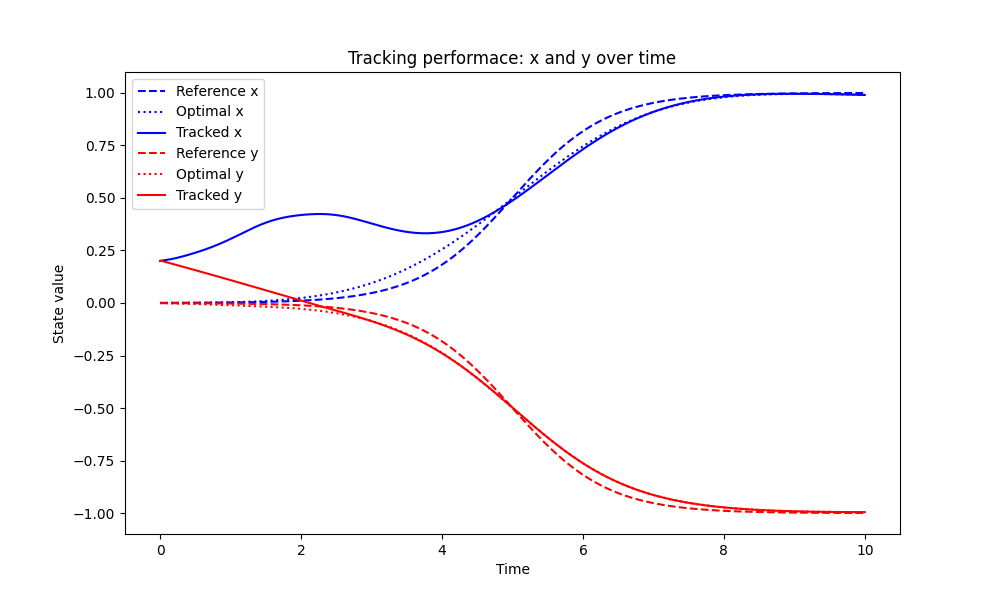
\includegraphics[width=1\textwidth]{pictures/tracking_xy.png}\hfill \\
  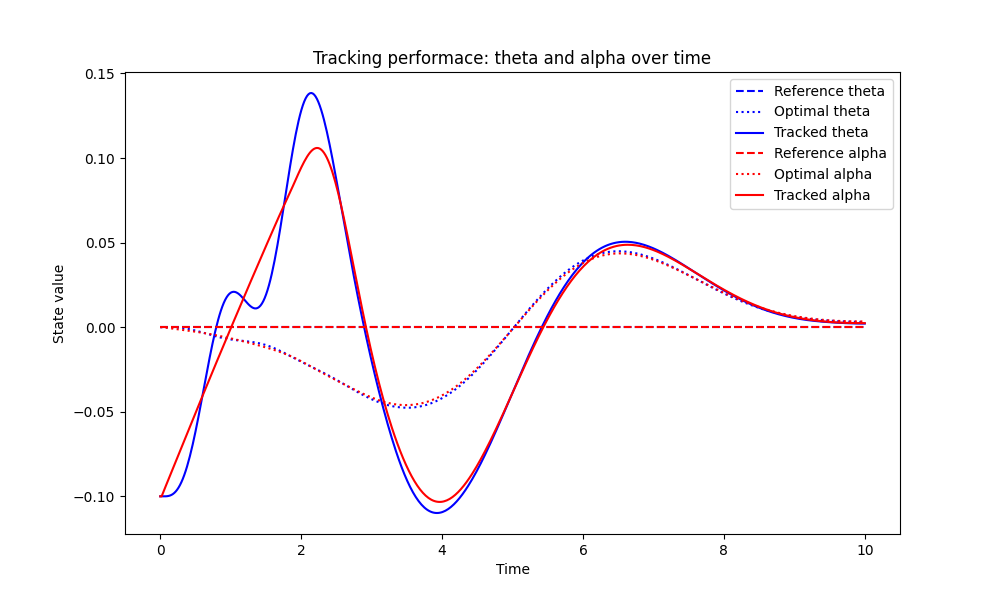
\includegraphics[width=1\textwidth]{pictures/tracking_theta_alpha.png}\hfill
  \caption{configuration tracking.}
  \label{fig:Reference trajectory}
\end{figure}

\begin{figure}[H]
  \centering
  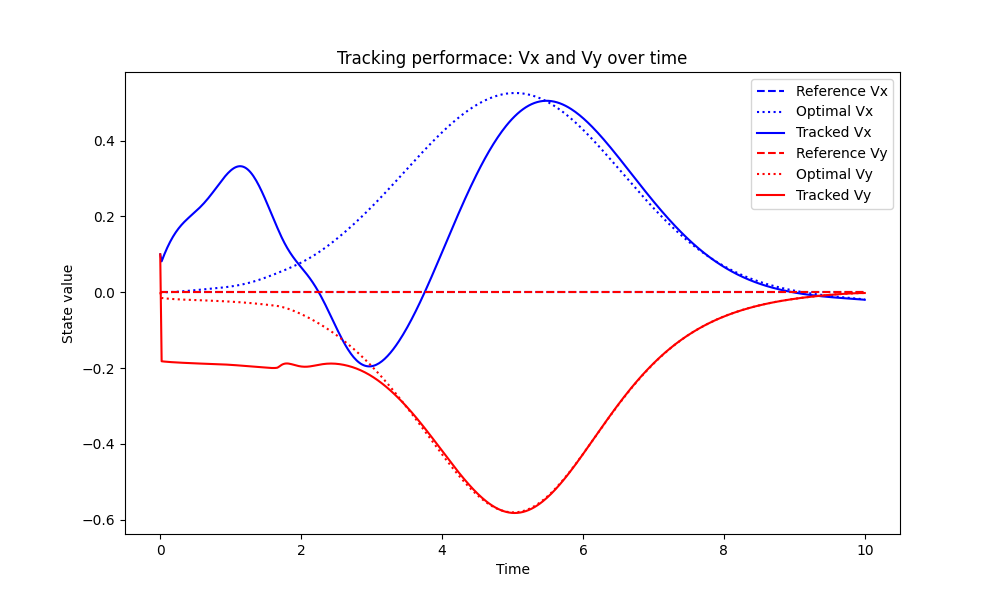
\includegraphics[width=1\textwidth]{pictures/tracking_vx_vy.png}\hfill \\
  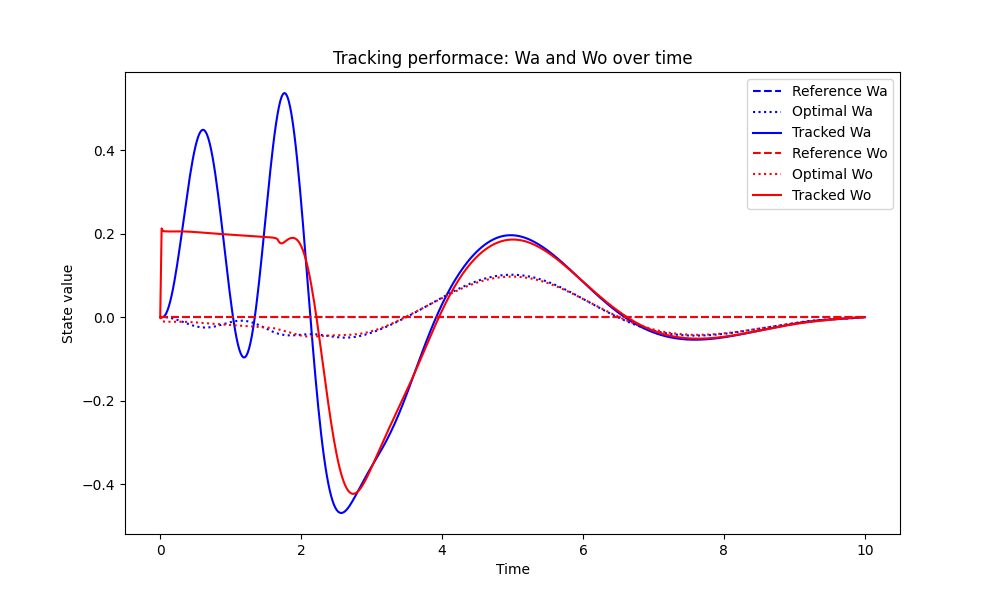
\includegraphics[width=1\textwidth]{pictures/tracking_omega.png}\hfill
  \caption{velocity tracking.}
  \label{fig:Reference trajectory}
\end{figure}

\begin{figure}[H]
  \centering
  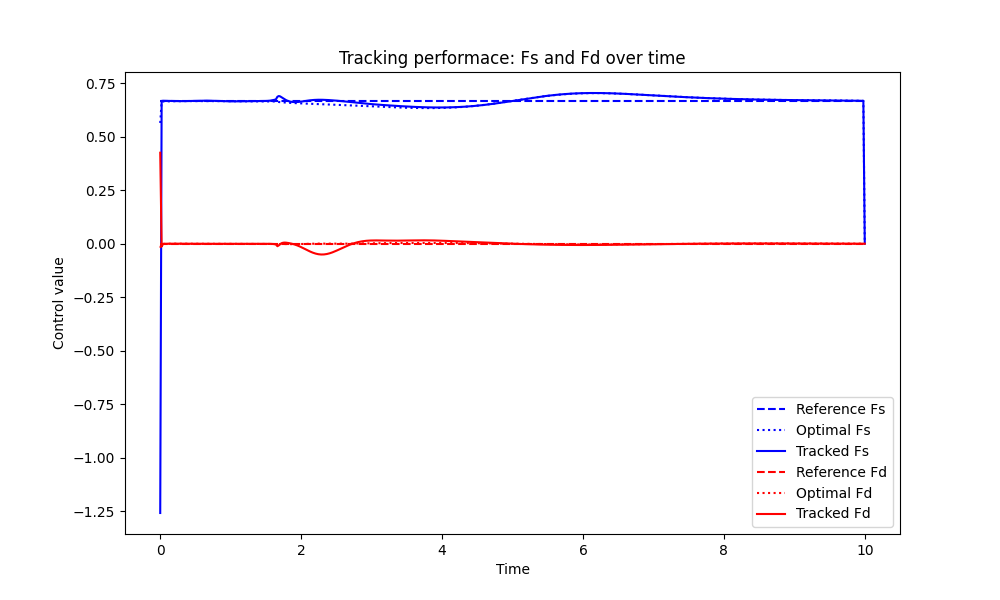
\includegraphics[width=1\textwidth]{pictures/tracking_input.png}\hfill \\
  \caption{input tracking.}
  \label{fig:Reference trajectory}
\end{figure}
